\section{Introduction}
Modeling is a powerful tool in synthetic biology. It can provide us with an important engineering approach to characterize our pathways quantitatively and predict their performance, thus help us test and modify our design.

Through the dynamic model, we hope to gain insights of the characteristics of our whole circuit's dynamics. Several tools including ODEs and interpolation are employed.


\section{Method}

\begin{figure}[h]
\centering
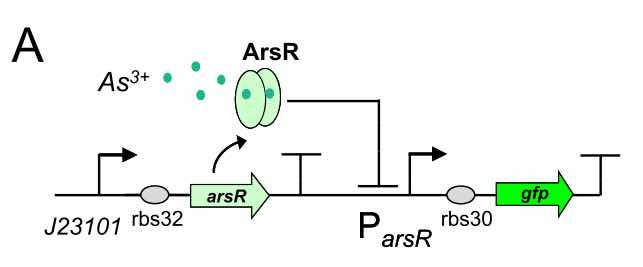
\includegraphics[width=12cm,height=5cm]{1}
\caption{Schematic diagram of plasmid1}
\end{figure}

At the beginning, on the plasmid\#1, the promoter $P_{arsR}$ isn't bound with ArsR, thus it is active. $ArsR$ and $smURFP$ are transcribed and translated under the control of the promoters $P_{arsR_u}$ and $P_{arsR_d}$, with subscript $u$ and $d$ representing upstream and downstream separately. The subscript $l$ of smURFP in the equation means leaky expression without the expression of $As^{3+}$. As ArsR is expressed gradually, it will bind with the promoter $P_{arsR}$ and make it inactive. \cite{pola2018novel}

\begin{equation}
P_{J23104} \stackrel{k_1}{\longrightarrow} P_{J23104}+ArsR
\end{equation}
\begin{equation}
P_{arsR_d} \stackrel{k_2}{\longrightarrow} P_{arsR_d} +smURFP_l
\end{equation}

\begin{equation}
ArsR+P_{arsR} \xrightleftharpoons[k_{-3}]{k_3}ArsR*P_{arsR} 
\end{equation} 

On the plasmid\#2, the fusion protein of dCas9 and RNAP(RNA polymerase) are produced after transcription and translation, and $sgRNA$ is produced after transcription.

\begin{equation}
P_{tet} \stackrel{k_{4}}{\longrightarrow} P_{tet} +dCas9*RNAP
\end{equation}
\begin{equation}
P_{tet} \stackrel{k_{5}}{\longrightarrow} P_{tet} +sgRNA
\end{equation}

\begin{figure}[h]
	\centering
	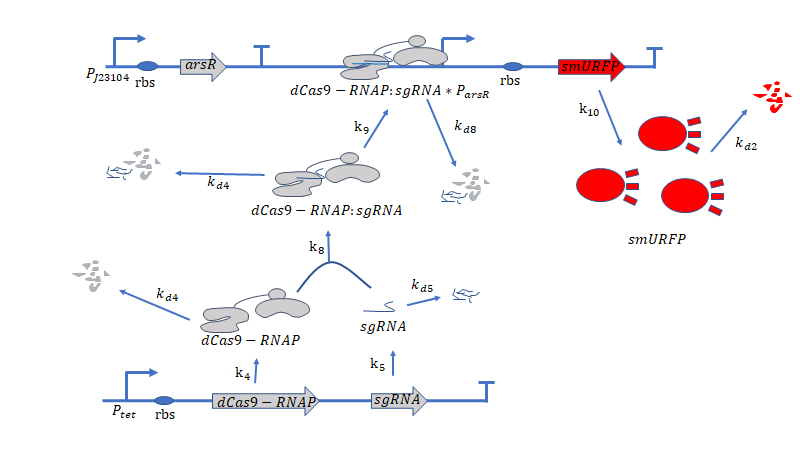
\includegraphics[width=12cm,height=5cm]{2}
	\caption{Schematic diagram of dCas9/RNAP}
\end{figure}

dCas9(*RNAP) can bind with its target DNA sequence without cutting, which is at the upstream of the promoter $P_{arsR_d}$. Simultaneously, dCas9 can lead RNAP to bind with the promoter $P_{arsR_d}$ and enhance the transcription of smURFP. However, because the promoter $P_{arsR_d}$ has already bound with ArsR, as a result, RNAP can't bind with the promoter $P_{arsR_d}$ .\cite{bikard2013programmable} \\ 

However, at the presence of $As^{3+}$, it can bind with ArsR, then dissociate ArsR and $P_{arsR_d}$, which makes the combination of RNAP and $P_{arsR_d}$ possible. \\

(Declaration: $[dCas9/RNAP] = [dCas9] = [RNAP]$;\\ $[P_{arsR_d}]=[P_{arsR_u}] = \frac{1}{2}[P_{arsR}]$ )

\begin{equation}
ArsR +As^{3+}\xrightleftharpoons[k_{-6}]{k_6}As^{3+}*ArsR
\end{equation}
\begin{equation}
ArsR*P_{arsR} +As^{3+}\xrightleftharpoons[k_{-7}]{k_7}P_{arsR}+ As^{3+}*ArsR
\end{equation}
\begin{equation}
dCas9*RNAP+sgRNA\xrightleftharpoons[k_{-8}]{k_8} dCas9*RNAP:sgRNA
\end{equation}
\begin{equation}
dCas9*RNAP:sgRNA+P_{arsR_d}\xrightleftharpoons[k_{-9}]{k_9} dCas9*RNAP:sgRNA*P_{arsR_d}
\end{equation}
\begin{equation}
dCas9*RNAP:sgRNA*P_{arsR_d}\stackrel{k_{10}}{\longrightarrow} dCas9*RNAP:sgRNA*P_{arsR_d}+smURFP
\end{equation}
\\
We then take degradation into account:\\
\begin{equation}
ArsR\stackrel{k_{d1}}{\longrightarrow}Ø
\end{equation}

\begin{equation}
smURFP\stackrel{k_{d2}}{\longrightarrow}Ø
\end{equation}


\begin{equation}
ArsR*P_{arsR}\stackrel{k_{d3}}{\longrightarrow}P_{arsR}
\end{equation}

\begin{equation}
As^{3+}*ArsR\stackrel{k_{d4}}{\longrightarrow}As^{3+}
\end{equation}

\begin{equation}
dCas9*RNAP\stackrel{k_{d5}}{\longrightarrow}Ø
\end{equation}

\begin{equation}
sgRNA\stackrel{k_{d6}}{\longrightarrow}Ø
\end{equation}

%\begin{equation}
%dCas9-RNAP:sgRNA\stackrel{k_{d7}}{\longrightarrow}dCas9-RNAP
%\end{equation}

\begin{equation}
dCas9*RNAP:sgRNA\stackrel{k_{d7}}{\longrightarrow}Ø
\end{equation}

%\begin{equation}
%dCas9-RNAP:sgRNA*P_{arsR}\stackrel{k_{d8}}{\longrightarrow}dCas9-RNAP+P_{arsR}
%\end{equation}

\begin{equation}
dCas9*RNAP:sgRNA*P_{arsR}\stackrel{k_{d8}}{\longrightarrow}P_{arsR}
\end{equation}
\\

We can now consider each reaction(not following the order above). We will use v as an arbitrary variable, simply there to denote a rate of reaction. The r0x notation will be used later in the programming to remove clutter from the code. The several complexes involved:$ArsR*P_{arsR}$ , $As^{3+}*ArsR$, dCas9-RNAP, dCas9*RNAP:sgRNA, $dCas9*RNAP:sgRNA*P_{arsR}$, are respectively abbreviated as $cplx_1$, $cplx_2$, $cplx_3$, $cplx_4$, $cplx_5$.\\
(1)Production of protein ArsR (r01):
\begin{displaymath}
v=k_1[P_{J23104}]
\end{displaymath}
(2)Degration of ArsR protein (r02):
\begin{displaymath}
v=-k_{d1}[ArsR]
\end{displaymath}
Note that this rate will be negative. This is because it will be decreasing the concentration of the ArsR protein . We can now put them together, to form an ordinary differential equation (ODE) for the rate of change in ArsR protein concentration.
\begin{equation}
\frac{d[ArsR]}{dt}=k_1[P_{arsR}]-k_{d1}[P_{arsR}][ArsR]\tag{1}
\end{equation}
(3)Production of protein smURFP under unbound promoter (r03):
\begin{displaymath}
v=k_2[P_{arsR}]
\end{displaymath}
(4)Production of protein smURFP under dCas9*RNAP:sgRNA-bound promoter (r04):
\begin{displaymath}
v=k_{10}[cplx_5]
\end{displaymath}
(5)Degration of smURFP protein (r05):
\begin{displaymath}
v=-k_{d2}[smURFP]
\end{displaymath}
These two come together to form an ODE for the rate of change in smuRFP protein concentration:
\begin{equation}
\frac{d[smURFP]}{dt}=k_2[P_{arsR}]+k_{10}[cplx_5]-k_{d2}[smuRFP]\tag{2}
\end{equation}
(6)Combination of ArsR protein and $P_{arsR}$ promoter(r06):
\begin{displaymath}
v=k_3[ArsR][P_arsR]
\end{displaymath}
(7)Combination of $As^{3+}$ and ArsR protein bound with $P_{arsR}$ promoter , also dissociation of ArsR protein and $P_{arsR}$ promoter(r07):
\begin{displaymath}
v=k_7[As^{3+}][cplx_1]
\end{displaymath}
(8)Degration of ArsR protein in the  $ArsR*P_{arsR}$ complex(r08):
\begin{displaymath}
v=-k_{d3}[cplx_1]
\end{displaymath}
Similarly, these three form the ODE for the rate of change in  $ArsR*P_{arsR}$ concentration.  :
\begin{equation}
\frac{d[cplx_1]}{dt}=k_3[ArsR][P_{arsR}]-k_7[As^{3+}][[cplx_1]-k_{d3}[cplx_1] \tag{3}
\end{equation}
Note that, in this ODE, $k_7$ will be negative. This is because it will be decreasing the concentration of  $ArsR*P_{arsR}$ complex.\\
(9)Production of dCas9-RNAP fusion protein (r09):
\begin{displaymath}
v=k_4[P_{tet}]
\end{displaymath}
(10)Degration of dCas9-RNAP fusion protein(r010):
\begin{displaymath}
v=k_{d5}[cplx_3]
\end{displaymath}
(11)Combination of dCas9-RNAP fusion protein and it's sgRNA(r011):
\begin{displaymath}
v=k_{8}[cplx_3][sgRNA]
\end{displaymath}
These three form the ODE for the rate of change in $dCas9-RNAP$ concentration.
\begin{equation}
\frac{d[cplx_3]}{dt}=k_4[P_{tet}]-k_{8}[cplx_3][sgRNA]-k_{d5}[cplx_3] \tag{4}
\end{equation}
Note that, in this ODE, $k_8$ will be negative. This is because it will be decreasing the concentration of  $dCas9-RNAP$ complex.\\
(12)Production of sgRNA (r012):
\begin{displaymath}
v=k_5[P_{tet}]
\end{displaymath}
(13)Degration of sgRNA(r013)
\begin{displaymath}
v=k_{d6}[sgRNA]
\end{displaymath}
These two plus r010 come together to form an ODE for the rate of change in sgRNA concentration:
\begin{equation}
\frac{d[sgRNA]}{dt}=k_5[P_{tet}]-k_{8}[cplx_3][sgRNA]-k_{d6}[sgRNA] \tag{5}
\end{equation}
Similarly, in this ODE, $k_8$ will be negative. This is because it will be decreasing the concentration of sgRNA complex.\\
(14)Combination of $As^{3+}$ and ArsR protein (r014):
\begin{displaymath}
v=k_{6}[As^{3+}][ArsR]
\end{displaymath}
(15)Degration of ArsR protein in the  $As^{3+}*ArsR$ complex(r015):
\begin{displaymath}
v=-k_{d6}[As^{3+}*ArsR]
\end{displaymath}
These two plus r06 come together to form an ODE for the rate of change in $As^{3+}*ArsR$  concentration and an ODE for the rate of change in $As^{3+}$ concentration:
\begin{equation}
\frac{d[cplx_2]}{dt}=k_{6}[As^{3+}][ArsR]+k_7[As^{3+}][cplx_1]-k_{d4}[cplx_2] \tag{6}
\end{equation}
Note that, in this ODE, $k_7$ will be positive,different from ODE(3). This is because it will be increasing the concentration of  $As^{3+}*ArsR$ complex.\\
\begin{equation}
\frac{d[cplx_2]}{dt}=-k_{6}[As^{3+}][ArsR]-k_7[As^{3+}][cplx_1] \tag{7}
\end{equation}
(16)Combination of dCas9-RNAP:sgRNA complex and $P_{arsR}$ promoter (r016):
\begin{displaymath}
v=k_{9}[cplx_4][P_{arsR}]
\end{displaymath}
(17)Degration of dCas9-RNAP:sgRNA complex (r017): 
\begin{displaymath}
v=-k_{d7}[cplx_4]
\end{displaymath}
These two plus r010 come together to form an ODE for the rate of change in dCas9-RNAP:sgRNA complex concentration:
\begin{equation}
\frac{d[cplx_4]}{dt}=k_{8}[cplx_3][sgRNA]-k_{9}[cplx_4][P_{arsR}]-k_{d7}[cplx_4]\tag{8}
\end{equation}
Note that, in this ODE, $k_8$ will be positive,different from ODE(4). This is because it will be decreasing the concentration of dCas9-RNAP:sgRNA complex.\\
(18))Degration of dCas9-RNAP:sgRNA complex in $dCas9-RNAP:sgRNA*P_{arsR}$ compex(r018):
\begin{displaymath}
v=-k_{d8}[cplx_5]
\end{displaymath}
This reaction and r016 come together to form an ODE for the rate of change in $dCas9-RNAP:sgRNA*P_{arsR}$ complex concentration:
\begin{equation}
\frac{d[cplx_5]}{dt}=k_{9}[cplx_4][P_{arsR}]-k_{d8}[cplx_5]\tag{9}
\end{equation} 
At last, the ODEs for the rate of change in three promoter:
\begin{equation}
\frac{d[P_{J23104}]}{dt}=0\tag{10}
\end{equation} 
\begin{equation}
\frac{d[P_{ArsR}]}{dt}=0\tag{11}
\end{equation} 
\begin{equation}
\frac{d[P_{tet}]}{dt}=0\tag{12}
\end{equation} 
Altogether, we have 8 ODEs:
\begin{equation}
\frac{d[ArsR]}{dt}=k_1[P_{arsR}]-k_{d1}[P_{arsR}][ArsR]\tag{1}
\end{equation}
\begin{equation}
\frac{d[smURFP]}{dt}=k_2[P_{arsR}]+k_{10}[cplx_5]-k_{d2}[smuRFP]\tag{2}
\end{equation}
\begin{equation}
\frac{d[cplx_1]}{dt}=k_3[ArsR][P_{arsR}]-k_7[As^{3+}][[cplx_1]-k_{d3}[cplx_1] \tag{3}
\end{equation}
\begin{equation}
\frac{d[cplx_3]}{dt}=k_4[P_{tet}]-k_{8}[cplx_3][sgRNA]-k_{d5}[cplx_3] \tag{4}
\end{equation}
\begin{equation}
\frac{d[sgRNA]}{dt}=k_5[P_{tet}]-k_{8}[cplx_3][sgRNA]-k_{d6}[sgRNA] \tag{5}
\end{equation}
\begin{equation}
\frac{d[cplx_2]}{dt}=k_{6}[As^{3+}][ArsR]+k_7[As^{3+}][cplx_1]-k_{d4}[cplx_2] \tag{6}
\end{equation}
\begin{equation}
\frac{d[cplx_2]}{dt}=-k_{6}[As^{3+}][ArsR]-k_7[As^{3+}][cplx_1] \tag{7}
\end{equation}
\begin{equation}
\frac{d[cplx_4]}{dt}=k_{8}[cplx_3][sgRNA]-k_{9}[cplx_4][P_{arsR}]-k_{d7}[cplx_4]\tag{8}
\end{equation}
\begin{equation}
\frac{d[cplx_5]}{dt}=k_{9}[cplx_4][P_{arsR}]-k_{d8}[cplx_5]\tag{9}
\end{equation} 
\begin{equation}
\frac{d[P_{J23104}]}{dt}=0\tag{10}
\end{equation} 
\begin{equation}
\frac{d[P_{ArsR}]}{dt}=0\tag{11}
\end{equation} 
\begin{equation}
\frac{d[P_{tet}]}{dt}=0\tag{12}
\end{equation} 
\\\\
\begin{table}[htbp]
	\centering
	\caption{\label {tab:test} Parameters}
	\begin{tabular}{cccccccccccccccccc}
		\toprule
		Rate constants & Value& units \\
		\midrule
		k1 & 1.999e-5 &1/s & Berset et al. \\
	k2 & 3.312e-6 &1/s & Berset et al.\\
	k3 & 3.3e7    & 1/M &Berset et al.   \\
	k4 &1.995e-5 &1/s & Estimated to be the same as in comparison to k1\\
	k5 & 3.312e-6 &1/s&Estimated to be the same as in comparison to k2\\
	k6 &1.66e7   &1/M & Berset et al.  \\
	k7  &1.26e4 &1/s & Berset et al. \\
	k8&1.6e-2& 1/s & 2017igem Munich\\
	k9 &1.66e-5&1/s&  2017igem Munich\\ 
	k10&4e-5&1/s & Estimated to be slow in comparison to k2 \\
	kd1 & 3.07e-3&1/s & Berset et al.\\
	kd2&1e-5&1/s & Berset et al.\\
	kd3&1e-3&1/s  & Berset et al.\\
	kd4&1.53e-3&1/s  & Berset et al.\\
	kd5 & 2e-2&1/s & Estimated to be fast in comparison to kd1\\
	kd6&7.62e-3&1/s&  Estimated according to Berset et al.\\
	kd7& 1e-2&1/s&  Estimated to be slow in comparison to kd5\\
	kd8&1e-1&1/s&  Estimated to be slow in comparison to kd7\\			
		\bottomrule
	\end{tabular}
\end{table}



\subsection{simulation }
\begin{figure}[h]
	\centering
	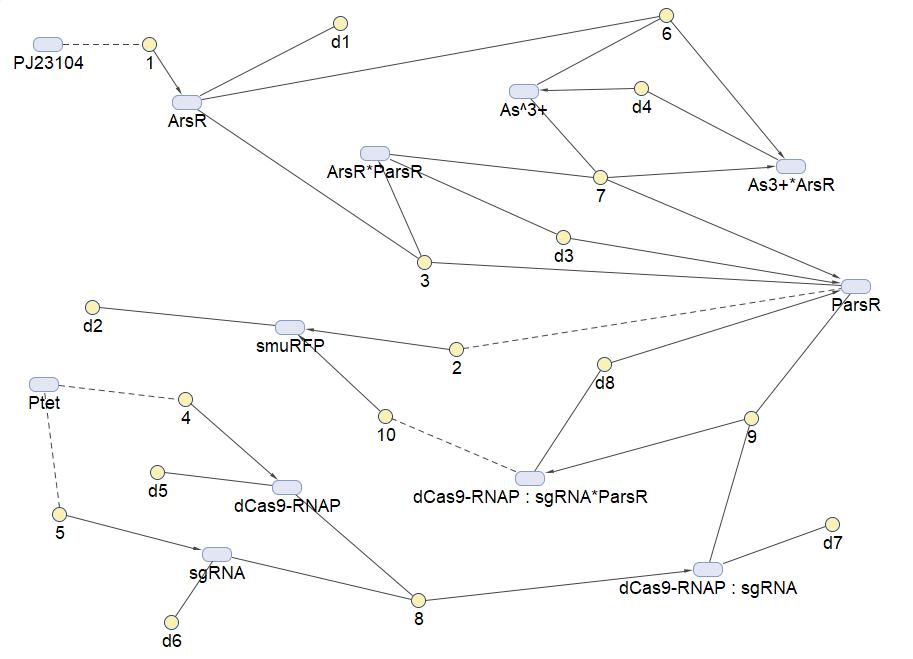
\includegraphics[width=10cm,height=7cm]{screenshot003}	
	\caption{reaction map generated from the reaction set above using SimBiology Toolbox}
\end{figure}
SimBiology toolbox provides functions for modeling, simulating, and analyzing biochemical pathways on basis of the powerful computing engine of Matlab.

\begin{figure}[h]
	\centering
	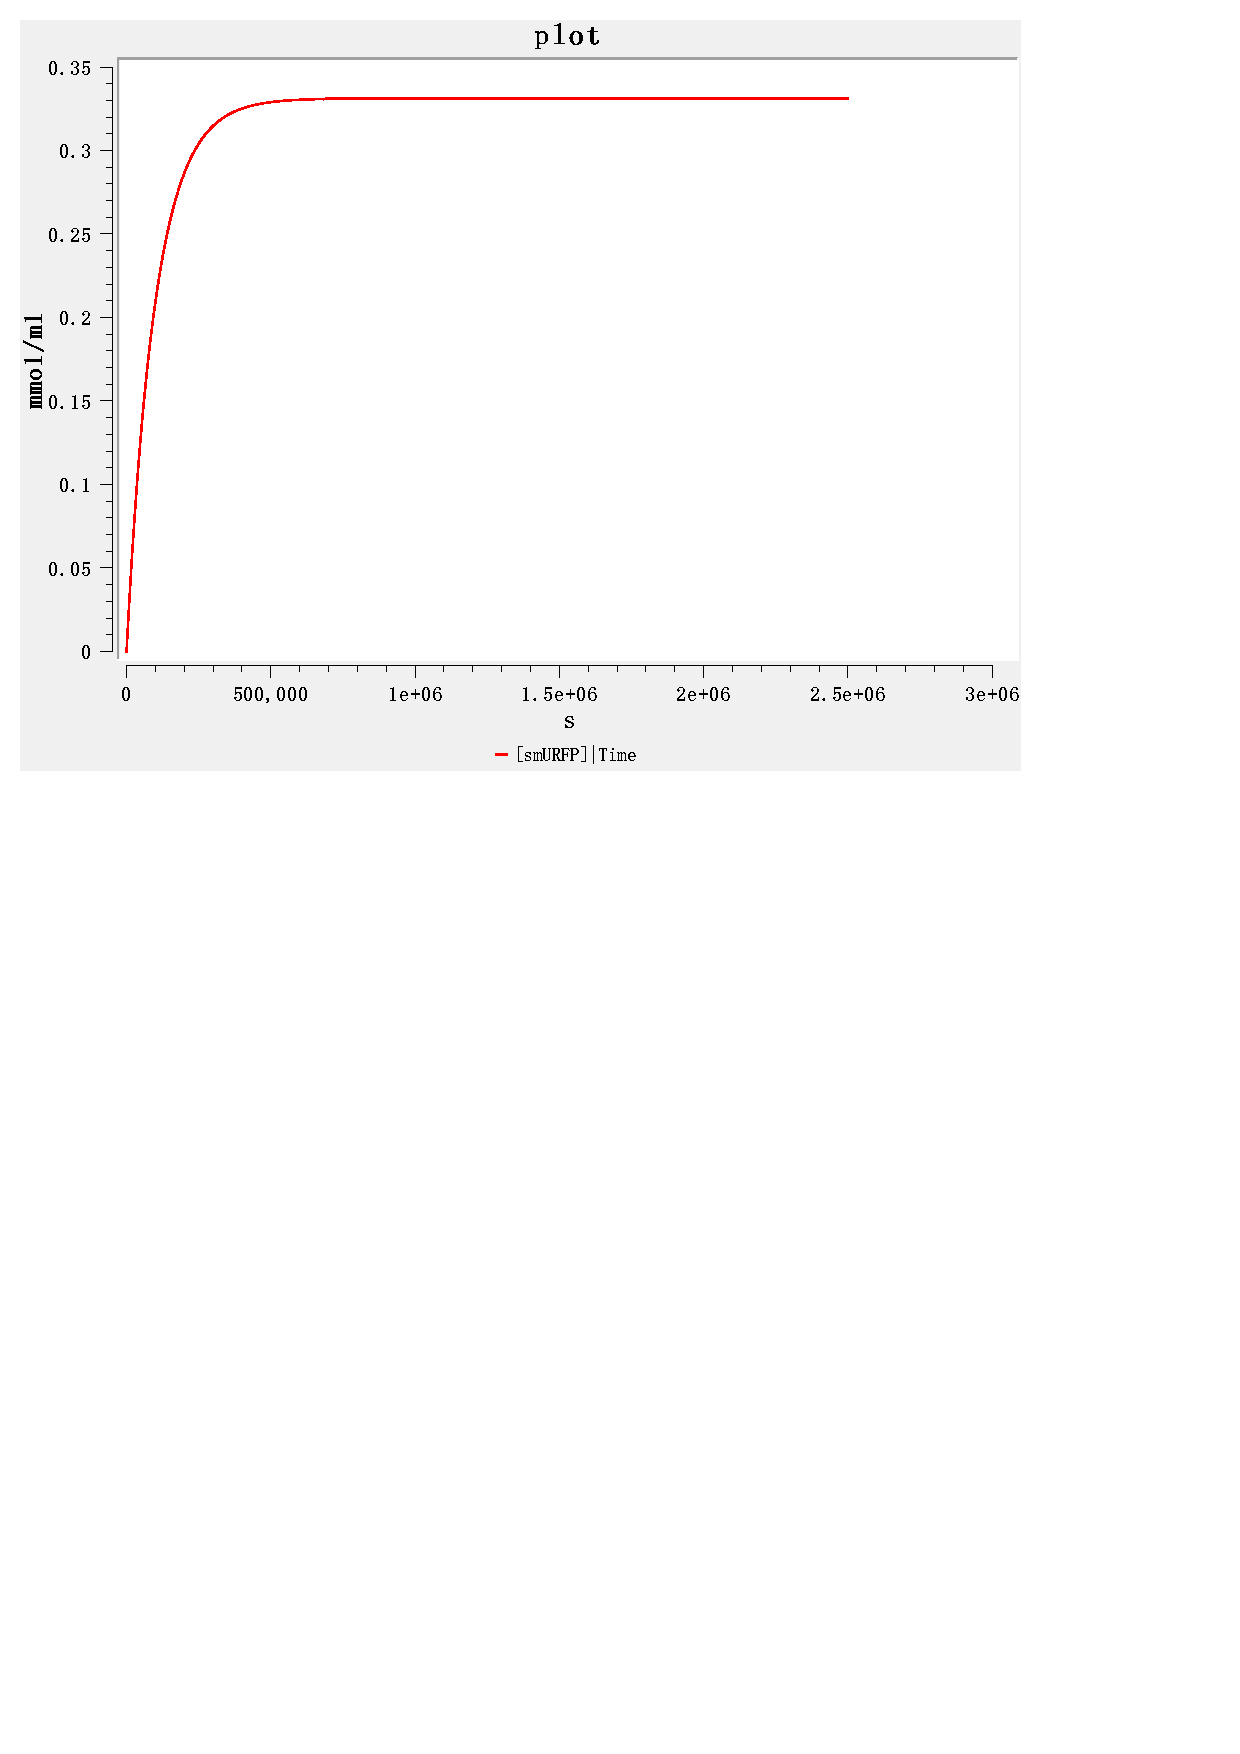
\includegraphics[width=10cm,height=10cm]{smuRFP}
	\caption{Schematic diagram of smURFP fluorescence by COPASI}
\end{figure}



COPASI is freeware developed withcollaboration of VBI and EMLR. It provides
almost the same functions as SimBiology, though not quite powerful. But compared with SimBiology, it provides a friendly user interface for model analysis, such as parameter estimation,and parameter scan.

Through the figure, we can see that the smURFP fluorescence gradually increased and then reached a steady state after a period of time  in the presence of arsenic ions.








